% Lectures/lec_3.tex
\lecture{3}{}{Derivatives, Root Finding, and Minimization}



\subsection{A Note on Notation: Derivatives as Linear Operators}

To proceed, we must first establish a clear and consistent notation for derivatives, treating them as linear operators that describe the local change of a function.

\begin{notation}
	Let \(f: \mathbb{R}^n \to \mathbb{R}^m\) be a differentiable function. The \textbf{Jacobian} of \(f\) at a point \(\vec{x}\) is the unique \(m \times n\) matrix, denoted \(\pdv{f}{\vec{x}}\), that satisfies the first-order Taylor approximation:
	\begin{equation}
		f(\vec{x} + \delta\vec{x}) \approx f(\vec{x}) + \left.\pdv{f}{\vec{x}}\right|_{\vec{x}} \delta\vec{x}
	\end{equation}
	This convention ensures that the chain rule for Jacobians works as expected with standard matrix multiplication. If we have \(h(\vec{z}) = f(g(\vec{z}))\), then:
	\[
		\pdv{h}{\vec{z}} = \left.\pdv{f}{\vec{y}}\right|_{g(\vec{z})} \pdv{g}{\vec{z}}
	\]
	For a scalar-valued function \(f: \mathbb{R}^n \to \mathbb{R}\), its Jacobian \(\pdv{f}{\vec{x}}\) is a \(1 \times n\) row vector. For convenience, we define the \textbf{gradient} vector, \(\nabla f(\vec{x})\), as the transpose of the Jacobian.
	\begin{align*}
		\nabla f(\vec{x}) & := \left(\pdv{f}{\vec{x}}\right)^{\top} \quad (\text{an } n \times 1 \text{ column vector}) \\
	\end{align*}
	The \textbf{Hessian} matrix is the Jacobian of the gradient, resulting in an \(n \times n\) matrix of second partial derivatives.
	\begin{align*}
		\nabla^2 f(\vec{x}) & := \pdv{}{\vec{x}} (\nabla f(\vec{x})) = \pdv{^2 f}{\vec{x}^2} \quad (\text{an } n \times n \text{ matrix})
	\end{align*}
	With this, the second-order Taylor expansion of a scalar function is:
	\begin{equation}
		f(\vec{x} + \delta\vec{x}) \approx f(\vec{x}) + (\nabla f(\vec{x}))^{\top}\delta\vec{x} + \frac{1}{2}\delta\vec{x}^{\top} (\nabla^2 f(\vec{x})) \delta\vec{x}
	\end{equation}
\end{notation}

\subsection{Root Finding}

A fundamental problem in numerical methods is root finding: for a given function \(g: \mathbb{R}^n \to \mathbb{R}^n\), find a point \(\vec{x}^*\) such that \(g(\vec{x}^*) = \vec{0}\).

\begin{eg}
	Finding the equilibrium point of a dynamical system \(\dot{\vec{x}} = f(\vec{x})\) is a root-finding problem. Similarly, as we saw last lecture, solving the implicit equation in a Backward Euler step, \(\vec{x}_{k+1} - \vec{x}_k - h f(\vec{x}_{k+1}) = 0\), is also a root-finding problem for \(\vec{x}_{k+1}\).
\end{eg}

\subsubsection{Fixed-Point Iteration}

A closely related problem is finding a \textbf{fixed point}, i.e., an \(\vec{x}^*\) such that \(g(\vec{x}^*) = \vec{x}^*\). We can always convert a root-finding problem \(r(\vec{x}) = 0\) to a fixed-point problem by defining \(g(\vec{x}) = \vec{x} - r(\vec{x})\).

The simplest method for finding a fixed point is \textbf{fixed-point iteration}:
\[
	\vec{x}_{k+1} = g(\vec{x}_k)
\]
This method is only guaranteed to converge if the fixed point is stable (i.e., \(| \text{eig}(\pdv{g}{\vec{x}})| < 1\)) and the initial guess is within the basin of attraction. The convergence rate is typically linear, which can be quite slow.

\subsubsection{Newton's Method}

A much more powerful and faster method is \textbf{Newton's method}. It works by iteratively solving a linearized version of the root-finding problem.
Given a guess \(\vec{x}_k\), we seek a correction \(\delta\vec{x}\) such that \(g(\vec{x}_k + \delta\vec{x}) = \vec{0}\). We linearize \(g\) around \(\vec{x}_k\):
\[
	g(\vec{x}_k + \delta\vec{x}) \approx g(\vec{x}_k) + \left.\pdv{g}{\vec{x}}\right|_{\vec{x}_k} \delta\vec{x} = \vec{0}
\]
Solving for the correction \(\delta\vec{x}\) gives the Newton step:
\begin{equation}
	\delta\vec{x} = - \left(\pdv{g}{\vec{x}}\right)^{-1} g(\vec{x}_k)
\end{equation}
The next guess is then \(\vec{x}_{k+1} = \vec{x}_k + \delta\vec{x}\). This process is repeated until convergence.

\begin{algorithm}[H]
  \caption{Newton's Method for Root Finding}
	\DontPrintSemicolon
	\KwIn{Function \(g(\vec{x})\), initial guess \(\vec{x}_0\), tolerance \(\epsilon\)}
	\KwOut{Root \(\vec{x}^*\)}
	\BlankLine
	\(\vec{x}_k \leftarrow \vec{x}_0\) \;
	\While{\(\|\vec{g}(\vec{x}_k)\| > \epsilon\)}{
	Compute Jacobian \(\mat{J} = \pdv{g}{\vec{x}}|_{\vec{x}_k}\) \;
	Solve the linear system \(\mat{J}\delta\vec{x} = -g(\vec{x}_k)\) for \(\delta\vec{x}\) \;
	\(\vec{x}_{k+1} \leftarrow \vec{x}_k + \delta\vec{x}\) \;
	}
	\Return \(\vec{x}_k\) \;
	\caption{Newton's Method}
\end{algorithm}

\begin{code}[Julia Notebook: Root Finding for Backward Euler]
	The `root-finding.ipynb` notebook provides a perfect comparison of fixed-point iteration and Newton's method. Both are used to solve the Backward Euler equation for the pendulum. The notebook plots the error (norm of the residual) at each iteration for both methods.
	\begin{itemize}
		\item \textbf{Fixed-point iteration} shows a slow, steady, linear decrease in error on a semi-log plot. It takes many iterations to reach high precision.
		\item \textbf{Newton's method} exhibits its characteristic \textbf{quadratic convergence}. The error decreases extremely rapidly, with the number of correct digits roughly doubling at each step. It typically converges to machine precision in just a few iterations.
	\end{itemize}
	This demonstrates the power of Newton's method. While each step is more expensive (requiring a Jacobian and a linear solve, is of the order \(O(n^3)\)), the drastically fewer iterations required make it far more efficient overall.
\end{code}

\subsection{Unconstrained Minimization}

We now turn to the problem of finding a local minimum of a smooth scalar function \(f: \mathbb{R}^n \to \mathbb{R}\).
A \textbf{first-order necessary condition} for a point \(\vec{x}^*\) to be a local minimum is that the gradient vanishes:
\begin{equation}
	\nabla f(\vec{x}^*) = \vec{0}
\end{equation}
This turns the minimization problem into a root-finding problem on the gradient! We can directly apply Newton's method.

\begin{definition}[Newton's Method for Minimization]
	To find a point where \(\nabla f(\vec{x}) = \vec{0}\), we apply the Newton's method recipe. The "function" we are finding the root of is now \(\nabla f(\vec{x})\). The "Jacobian" of this function is the Hessian, \(\nabla^2 f(\vec{x})\). The Newton step is therefore:
	\begin{equation}
		\delta\vec{x} = - (\nabla^2 f(\vec{x}))^{-1} \nabla f(\vec{x})
	\end{equation}
	The intuition here is that we are fitting a quadratic model to the function at the current point (based on the second-order Taylor expansion) and then jumping directly to the minimum of that quadratic model.
\end{definition}

However, there are pitfalls. The condition \(\nabla f(\vec{x}^*) = \vec{0}\) applies to local maxima and saddle points as well as minima. A standard Newton step can easily converge to the wrong type of point.

A \textbf{second-order sufficient condition} for \(\vec{x}^*\) to be a strict local minimum is that \(\nabla f(\vec{x}^*) = \vec{0}\) and the Hessian \(\nabla^2 f(\vec{x}^*)\) is \textbf{positive definite} (all its eigenvalues are positive).
A Newton step is a \textit{descent direction} (i.e., a step that decreases the function value) if and only if the Hessian is positive definite. If the Hessian is negative definite (at a maximum), Newton's method becomes an \textit{ascent} method.

\begin{code}[Julia Notebook: The Pitfall of Standard Newton's Method]
	The `minimization.ipynb` notebook clearly illustrates this problem. It attempts to minimize the function \(f(x) = x^4 + x^3 - x^2 - x\).
	\begin{center}
		% Figures/minimization_plot.tex
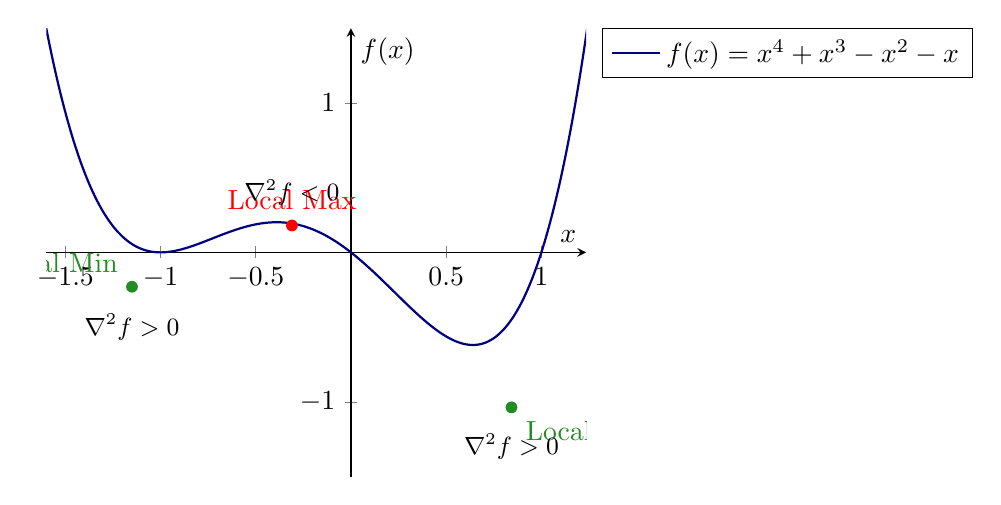
\begin{tikzpicture}
    \begin{axis}[
        axis lines=middle,
        xlabel=$x$,
        ylabel={$f(x)$},
        samples=200,
        domain=-1.75:1.25,
        ymin=-1.5,
        ymax=1.5,
        legend pos=outer north east,
        ]
        \addplot[thick, NavyBlue, smooth] {x^4 + x^3 - x^2 - x};
        \addlegendentry{$f(x) = x^4 + x^3 - x^2 - x$}

        % Minima and Maxima
        \node[circle, fill=ForestGreen, inner sep=1.5pt, label={[ForestGreen]below right:Local Min}] at (axis cs:0.843, -1.037) {};
        \node[circle, fill=ForestGreen, inner sep=1.5pt, label={[ForestGreen]above left:Local Min}] at (axis cs:-1.15, -0.23) {};
        \node[circle, fill=Red, inner sep=1.5pt, label={[Red]above:Local Max}] at (axis cs:-0.31, 0.18) {};

        % Hessian signs
        \node[font=\small] at (axis cs:0.843, -1.3) {$\nabla^2 f > 0$};
        \node[font=\small] at (axis cs:-1.15, -0.5) {$\nabla^2 f > 0$};
        \node[font=\small] at (axis cs:-0.31, 0.4) {$\nabla^2 f < 0$};
    \end{axis}
\end{tikzpicture}

	\end{center}
	When an initial guess of \(x_0=0\) is used, the Hessian \(\nabla^2 f(0)\) is negative. The notebook shows that the standard Newton step moves from \(x=0\) towards the local maximum, not the minimum.
\end{code}

\subsubsection{Regularization (Damped Newton's Method)}

To fix this, we can \textbf{regularize} the Hessian. The goal is to modify the Hessian \(\mat{H} = \nabla^2 f(\vec{x})\) to ensure it is positive definite, thus guaranteeing a descent direction. A simple and effective method is Levenberg-Marquardt style damping:
\[
	\text{If } \mat{H} \text{ is not positive definite, replace it with } \mat{H}' = \mat{H} + \beta\mat{I}
\]
where \(\beta > 0\) is a damping parameter. We can increase \(\beta\) until \(\mat{H}'\) becomes positive definite. This has two effects:
\begin{enumerate}
	\item It guarantees the resulting step \(\delta\vec{x} = -(\mat{H}')^{-1}\nabla f(\vec{x})\) is a descent direction.
	\item As \(\beta \to \infty\), the step becomes \(\delta\vec{x} \approx -\frac{1}{\beta}\nabla f(\vec{x})\), which is a small step in the steepest descent direction.
\end{enumerate}
This method adaptively blends between the fast Newton step (when the function is locally convex) and the robust but slow gradient descent step (when it is not).

\begin{code}[Julia Notebook: Regularized Newton's Method]
	The notebook implements this regularization. When starting from \(x_0=0\), the algorithm detects the negative Hessian, adds damping, and computes a new step. The resulting step is now correctly pointed towards the local minimum. This demonstrates how regularization makes Newton's method a robust tool for nonlinear optimization.
\end{code}


\subsection{Supplementary Concepts}

We adopt the setting of unconstrained smooth optimization \(\min_{\vec{x}\in\mathbb{R}^n} f(\vec{x})\) with \(f\in C^2\) unless otherwise specified.

\subsubsection{Convexity and Strong Convexity}
\begin{definition}[Convex Function]
Let \(\mathcal{D} \subseteq \mathbb{R}^n\) be convex. A function \(f: \mathcal{D}\to\mathbb{R}\) is convex if for all \(\vec{x},\vec{y}\in\mathcal{D}\) and \(\theta\in[0,1]\):
\[
		f(\theta \vec{x} + (1-\theta)\vec{y}) \le \theta f(\vec{x}) + (1-\theta) f(\vec{y}).
\]
It is \emph{strictly convex} if the inequality is strict whenever \(\vec{x}\neq\vec{y}\) and \(\theta\in(0,1)\).
\end{definition}

\begin{definition}[Strong Convexity]
For \(m>0\), \(f\) is \(m\)-strongly convex if
\[
		f(\vec{y}) \ge f(\vec{x}) + \nabla f(\vec{x})^{\top}(\vec{y}-\vec{x}) + \frac{m}{2}\|\vec{y}-\vec{x}\|^2, \quad \forall \vec{x},\vec{y}.
\]
\end{definition}

\begin{theorem}[Second-Order Characterizations]
Assume \(f\in C^2\) on an open convex domain.
\begin{itemize}
	\item \(f\) convex \(\iff \nabla^2 f(\vec{x})\) is positive semidefinite (PSD) for all \(\vec{x}\).
	\item \(f\) \(m\)-strongly convex \(\iff \nabla^2 f(\vec{x}) \succeq m \mat{I}\) for all \(\vec{x}\) (i.e., all eigenvalues \(\ge m\)).
\end{itemize}
\end{theorem}

\begin{theorem}[Alternative Strong Convexity Characterizations]
Let \(f\) be differentiable and \(m>0\). The following are equivalent:
\begin{enumerate}
	\item \(f\) is \(m\)-strongly convex.
	\item For all \(\vec{x},\vec{y}\), \((\nabla f(\vec{x}) - \nabla f(\vec{y}))^{\top}(\vec{x}-\vec{y}) \ge m \|\vec{x}-\vec{y}\|^2.\)
	\item For all \(\vec{x},\vec{y}\), \(f(\vec{y}) \ge f(\vec{x}) + \nabla f(\vec{x})^{\top}(\vec{y}-\vec{x}) + \frac{m}{2}\|\vec{y}-\vec{x}\|^2.\)
\end{enumerate}
\end{theorem}

\paragraph{Consequences.} Strong convexity implies uniqueness of the global minimizer. Plain convexity only guarantees that any local minimum is global (but possibly non-unique). For \(L\)-smooth functions (gradient Lipschitz with constant \(L\)), gradient descent with step size \(\alpha\in (0,2/L)\) converges; if additionally \(m\)-strongly convex, the convergence is linear with rate \(1 - m/L\).

\subsubsection{Optimality Conditions (Unconstrained)}
Let \(f\in C^2\). A point \(\vec{x}^*\) is a (local) minimizer only if the following hold.
\begin{theorem}[First-Order Necessary Condition]
If \(\vec{x}^*\) is a local minimizer, then \(\nabla f(\vec{x}^*) = \vec{0}.\)
\end{theorem}

\begin{theorem}[Second-Order Necessary Condition]
If \(\vec{x}^*\) is a local minimizer and \(f\in C^2\), then \(\nabla f(\vec{x}^*) = 0\) and \(\nabla^2 f(\vec{x}^*)\) is PSD.
\end{theorem}

\begin{theorem}[Second-Order Sufficient Condition]
If \(\nabla f(\vec{x}^*) = 0\) and \(\nabla^2 f(\vec{x}^*)\) is positive definite (PD), then \(\vec{x}^*\) is a strict local minimizer. If \(\nabla^2 f(\vec{x}) \succeq m\mat{I}\) globally (\(m>0\)), then \(\vec{x}^*\) is the unique global minimizer.
\end{theorem}

\paragraph{Saddle Points.} If the Hessian has both positive and negative eigenvalues at a stationary point, Newton's method may be attracted there; regularization or negative curvature exploitation is needed to escape.

\subsubsection{Positive Definiteness, Cholesky Factorization, and On-the-Spot Padding}
\begin{definition}[Positive (Semi)Definiteness]
A symmetric matrix \(\mat{H}\in\mathbb{R}^{n\times n}\) is PSD if \(\vec{v}^\top \mat{H} \vec{v}\ge 0\) for all \(\vec{v}\); PD if the inequality is strict for all nonzero \(\vec{v}\).
\end{definition}

\paragraph{Cholesky Factorization.} A symmetric matrix \(\mat{H}\) is PD \(\iff\) it admits a (unique) Cholesky factorization \(\mat{H} = \mat{R}^\top \mat{R}\) with \(\mat{R}\) upper triangular with positive diagonal. Attempting Cholesky is therefore a practical test: breakdown (negative pivot) indicates loss of definiteness.


% \subsubsection{Quasi-Newton Methods}
% Pure Newton's method requires the exact Hessian (costly to form/invert) and can fail when \(\nabla^2 f\) is indefinite. Quasi-Newton methods build and update a symmetric positive definite approximation \(\mat{B}_k\approx \nabla^2 f(\vec{x}_k)\) (or its inverse) using only gradients.

% Define the step \(\vec{s}_k = \vec{x}_{k+1} - \vec{x}_k\) and gradient change \(\vec{y}_k = \nabla f(\vec{x}_{k+1}) - \nabla f(\vec{x}_k)\). The
% \emph{secant equation} enforces \(\mat{B}_{k+1} \vec{s}_k = \vec{y}_k\).

% \paragraph{DFP (Davidon--Fletcher--Powell) Update (Inverse Form).} Maintaining \(\mat{H}_k \approx (\nabla^2 f)^{-1}\):
% \[
% 	\mat{H}_{k+1} = \mat{H}_k + \frac{\vec{s}_k \vec{s}_k^{\top}}{\vec{s}_k^{\top}\vec{y}_k} - \frac{\mat{H}_k \vec{y}_k \vec{y}_k^{\top} \mat{H}_k}{\vec{y}_k^{\top} \mat{H}_k \vec{y}_k}.
% \]

% \paragraph{BFGS Update (Primal and Inverse).} Widely used due to robustness and superlinear convergence under standard assumptions.
% Primal form (approximate Hessian):
% \[
% 	\mat{B}_{k+1} = \mat{B}_k - \frac{\mat{B}_k \vec{s}_k \vec{s}_k^{\top} \mat{B}_k}{\vec{s}_k^{\top} \mat{B}_k \vec{s}_k} + \frac{\vec{y}_k \vec{y}_k^{\top}}{\vec{y}_k^{\top} \vec{s}_k}.
% \]
% Inverse form (maintaining \(\mat{H}_k = \mat{B}_k^{-1}\)):
% \[
% 	\mat{H}_{k+1} = \left(\mat{I} - \rho_k \vec{s}_k \vec{y}_k^{\top}\right) \mat{H}_k \left(\mat{I} - \rho_k \vec{y}_k \vec{s}_k^{\top}\right) + \rho_k \vec{s}_k \vec{s}_k^{\top}, \quad \rho_k = \frac{1}{\vec{y}_k^{\top} \vec{s}_k}.
% \]
% Positive definiteness is preserved if \(\vec{y}_k^{\top}\vec{s}_k > 0\). Line searches enforcing Wolfe curvature conditions guarantee this:
% \[
% 	f(\vec{x}_k + \alpha_k \vec{p}_k) \le f(\vec{x}_k) + c_1 \alpha_k \nabla f_k^{\top} \vec{p}_k, \quad \nabla f(\vec{x}_k+\alpha_k \vec{p}_k)^{\top} \vec{p}_k \ge c_2 \nabla f_k^{\top} \vec{p}_k
% \]
% with \(0 < c_1 < c_2 < 1\).

% \paragraph{SR1 (Symmetric Rank-1) Update.} Provides potentially better curvature information but does not guarantee PD:
% \[
% 	\mat{B}_{k+1} = \mat{B}_k + \frac{(\vec{y}_k - \mat{B}_k \vec{s}_k)(\vec{y}_k - \mat{B}_k \vec{s}_k)^{\top}}{(\vec{y}_k - \mat{B}_k \vec{s}_k)^{\top} \vec{s}_k}.
% \]
% Accepted only if denominator is sufficiently large in magnitude; otherwise the update is skipped.

% \paragraph{Limited-Memory BFGS (L-BFGS).} Stores only the most recent \(m\) pairs \((\vec{s}_i, \vec{y}_i)\) and applies them in a two-loop recursion to obtain \(\mat{H}_k \nabla f_k\) without forming the dense matrix. Standard for large-scale robotics parameter estimation and trajectory optimization problems.

% \paragraph{Convergence.} Under standard assumptions (\(f\) twice continuously differentiable, gradient Lipschitz, and bounded level sets), BFGS with an appropriate line search produces steps with \(\vec{y}_k^{\top}\vec{s}_k>0\) and achieves superlinear convergence to a nondegenerate minimizer. Quasi-Newton methods thus approximate Newton's speed without explicit Hessians.

% \paragraph{Relationship to Regularized Newton.} When \(\nabla^2 f\) is expensive or noisy (e.g., stochastic settings) BFGS acts as an implicit, data-driven regularizer, avoiding explicit Cholesky/damping while gradually learning curvature.
\newpage
